\chapter{Lie Theory for Rotations}
\label{ch:lie}

\begin{objectives}
\begin{itemize}
  \item Understand $\SO$ as a curved manifold with a flat tangent space, and why an estimator needs both.
  \item Use the exponential and logarithm maps, in matrix and quaternion form, and implement them robustly.
  \item Distinguish local (right) and global (left) perturbations, and move perturbations across a
        rotation with the adjoint.
  \item Define Jacobians of functions of rotations, derive the right Jacobian $\Jr$, and build a table
        of elementary Jacobians from which every Jacobian in the project can be assembled.
  \item Represent and propagate uncertainty on $\SO$, and test manifold Jacobians numerically.
\end{itemize}
\end{objectives}

This chapter is the mathematical core of the notes. Its conclusions fit in a few lines (the
$\bplus$/$\bminus$ operators of \cref{sec:boxplus} and the Jacobian table of \cref{tab:jacobians}),
but the reasoning behind them is what lets you derive any new Jacobian correctly. The treatment
follows the ``micro Lie theory'' of Solà et al.~\cite{sola2018micro}, specialized to $\SO$ with the
conventions of this project. Barfoot~\cite{barfoot2017state} covers the same material in greater depth.

% ------------------------------------------------------------------------------
\section{Why estimation needs Lie theory}

A Kalman filter represents uncertainty as a mean and a covariance and corrects the mean by adding
a vector. Both operations assume the state lives in a vector space. Attitude does not.
\begin{itemize}
  \item \textbf{Addition leaves the space.} If $\hat q$ is a unit quaternion and $\delta q$ a small
        4-vector, $\hat q + \delta q$ is generally not unit length. The same holds for rotation matrices.
  \item \textbf{Redundant parameters give singular covariances.} A unit quaternion has four
        components but three degrees of freedom. A $4\times4$ covariance of a unit quaternion must be
        singular along the radial direction, and keeping it exactly singular under rounding is hopeless.
  \item \textbf{Minimal parameters have singularities.} Euler angles (\cref{ch:rotations}) are minimal
        but singular at gimbal lock.
\end{itemize}

\begin{keyidea}[the Earth and its tangent planes]
The surface of the Earth is curved, yet a town map drawn on flat paper is perfectly accurate for a
walk across town. The map is the \emph{tangent plane} at your location. It works as long as you do
not walk too far, and when you move to a new town you draw a new map. An estimator does the same:
it stores the attitude on the curved space $\SO$ (the globe), and expresses small uncertainties and
corrections in the flat 3D tangent space at the current estimate (the town map). The exponential
map turns a step on the map into a point on the globe, and the logarithm map does the reverse.
\end{keyidea}

% ------------------------------------------------------------------------------
\section{Warm-up: rotations of the plane}
\label{sec:so2}

Every idea of this chapter appears, in its simplest form, for planar rotations $R(\theta)$. Work through them here; the rest of the chapter
asks only what changes in three dimensions.
\begin{itemize}
  \item \emph{The set.} Planar rotations form a circle: $R(\theta)$ and $R(\theta + 2\pi)$ are the same. The set is one-dimensional but curved, and it is
        not a vector space ($R(\alpha) + R(\beta)$ is not a rotation).
  \item \emph{The tangent space.} Differentiating $R(\theta)$ at $\theta = 0$ gives $\frac{\dd R}{\dd\theta}(0) = \begin{bmatrix}0 & -1\\ 1 & 0\end{bmatrix}$; every velocity at the
        identity is a multiple of this skew-symmetric matrix. The tangent space is a line, coordinatized by a single number.
  \item \emph{Exponential and logarithm.} $\exp\big(\theta\begin{bmatrix}0 & -1\\ 1 & 0\end{bmatrix}\big) = R(\theta)$ (sum the series, or solve
        $\dot R = R\begin{bmatrix}0&-1\\1&0\end{bmatrix}$), so ``$\Exp$'' maps an angle to a rotation. Its inverse ``$\Log$'' recovers the angle,
        $\theta = \atantwo(R_{21}, R_{11}) \in (-\pi, \pi]$, unique only up to the choice of branch.
  \item \emph{Perturbations.} An estimate $R(\hat\theta)$ with a small error is $R(\hat\theta)R(\delta\theta) = R(\hat\theta + \delta\theta)$. Because planar rotations commute,
        perturbing on the left or on the right is the same, and the error of the composition is just the sum of the angles.
  \item \emph{Jacobians.} The derivative of $\Exp$ is the identity (1), and nothing like the right Jacobian appears.
\end{itemize}
In the plane, therefore, one can simply estimate the angle as a scalar, as long as differences are wrapped to $(-\pi, \pi]$. In three dimensions
rotations do not commute, the identity $R(\alpha)R(\beta) = R(\alpha + \beta)$ fails for rotation vectors with different axes, and left and right
perturbations differ. Each of these failures produces a new object in this chapter: the adjoint, the Baker--Campbell--Hausdorff formula, and the
right and left Jacobians.

% ------------------------------------------------------------------------------
\section{Manifolds, groups and Lie groups}

\subsection{Manifolds and tangent spaces}

\index{manifold}
A smooth $n$-dimensional \term{manifold} is a space that looks like $\R^n$ near every point. Precisely, each point has a neighborhood that can be
mapped smoothly and invertibly onto an open set of $\R^n$ (a \emph{chart}), and where two charts overlap, the change of coordinates between them is
smooth. The surface of a sphere is a 2D manifold: latitude and longitude form a chart away from the poles, and a second chart covers the poles. A
manifold usually needs several charts; a single chart for the whole sphere does not exist, and neither does one for $\SO$, which is why every
three-number parameterization of attitude has singularities.

A \term{tangent vector} at a point $x$ of a manifold is the velocity $\dot\gamma(0)$ of a smooth curve $\gamma(t)$ through $\gamma(0) = x$. The tangent vectors
at $x$ form a vector space, the \term{tangent space} $T_x\mathcal M$, of the same dimension as the manifold. For a manifold that sits inside a larger
vector space (as $\SO$ sits inside $\R^{3\times3}$), tangent vectors are ordinary vectors tangent to the surface: the tangent plane of a sphere
in the Earth analogy.

\subsection{Groups}

\begin{definition}[Group]
\index{group}
A \term{group} $(\mathcal{G}, \circ)$ is a set with an operation $\circ$ that is associative, has an identity element $\mathcal{E}$
($\mathcal{E}\circ\mathcal{X} = \mathcal{X}\circ\mathcal{E} = \mathcal{X}$), and an inverse $\mathcal{X}\inv$ for every element
($\mathcal{X}\circ\mathcal{X}\inv = \mathcal{E}$).
\end{definition}

Commutativity is \emph{not} required. Examples: $(\R^n, +)$ (identity $0$, inverse $-x$); the invertible $n\times n$ matrices under multiplication;
$\SO$; the unit quaternions under the Hamilton product; the rigid motions $\SE$. A group can also \emph{act} on another set: a rotation acts on
vectors by $v \mapsto Rv$, and a rigid motion acts on points by $p \mapsto Rp + t$. These actions are how groups enter measurement models.

\begin{definition}[Lie group]
\index{Lie group}
A \term{Lie group} is a group that is also a smooth manifold, such that composition and inversion are smooth maps. A \emph{matrix Lie group} is a
Lie group whose elements are invertible matrices and whose operation is matrix multiplication.
\end{definition}

Being a group as well gives a Lie group a remarkable property. Multiplication by a fixed element maps a neighborhood of the identity smoothly onto
a neighborhood of that element: the space looks the same everywhere. All local calculus can therefore be done once, at the identity, and
carried to any other element by composition. This is what makes estimation on $\SO$ tractable: one tangent space (at the identity), one
exponential map, and one set of Jacobian formulas serve every attitude.

\begin{center}\small
\begin{tabular}{@{}l l l l@{}}
\toprule
Group & Elements & Dimension & Role in VIO \\
\midrule
$(\R^n, +)$ & vectors & $n$ & position, velocity, biases \\
$\mathrm{SO}(2)$ & planar rotations & 1 & toy examples \\
$\SO$ & $3\times3$ rotation matrices & 3 & attitude \\
$S^3$ & unit quaternions & 3 & attitude (double cover of $\SO$) \\
$\SE$ & rigid transformations & 6 & poses, extrinsics \\
\bottomrule
\end{tabular}
\end{center}

% ------------------------------------------------------------------------------
\section{The Lie algebra and tangent spaces}

Consider a smooth curve $R(t) \in \SO$ with $R(0) = I$. Differentiating $R\T R = I$ at $t = 0$ gives
$\dot R(0)\T + \dot R(0) = 0$: the velocity at the identity is skew-symmetric. The set of all such
velocities is the \emph{Lie algebra}
\begin{equation}
  \so = \{\, \Omega \in \R^{3\times3} : \Omega\T = -\Omega \,\} = \{\, \sx{\phi} : \phi \in \R^3 \,\},
\end{equation}
a three-dimensional vector space identified with $\R^3$ by the hat and vee maps,
$\phi\hatop = \sx{\phi}$ and $\sx{\phi}\veeop = \phi$. Unlike $\SO$ itself, the Lie algebra is flat:
we can add its elements, scale them, and put Gaussian distributions on them.

\index{Lie bracket}
The Lie algebra carries one more operation, the \emph{Lie bracket} (commutator) $[X, Y] = XY - YX$, which measures how much two infinitesimal
motions fail to commute. The commutator of two skew-symmetric matrices is skew-symmetric, and by \eqref{eq:skew-commutator}
\begin{equation}
  \big[\sx{a}, \sx{b}\big] = \sx{a \times b} .
\end{equation}
So $\so$ with its bracket is $\R^3$ with the cross product. The cross product, which is zero only for parallel vectors, is the infinitesimal
version of the non-commutativity of rotations: rotations about parallel axes commute, all others do not.

At a general point $R$, the tangent space consists of the velocities of curves through $R$. From
\eqref{eq:rdot}, every such velocity can be written in two ways,
\begin{equation}
  \dot R = R\,\sx{\omega_b} = \sx{\omega_w}\,R, \qquad \omega_w = R\,\omega_b,
\end{equation}
so the tangent space at $R$ can be identified with $\R^3$ in two ways: by a vector expressed in the
\emph{local} (body) frame, multiplying on the right, or by a vector expressed in the \emph{global}
(world) frame, multiplying on the left. This is the origin of the two perturbation conventions of
\cref{sec:perturbations}. The project uses the local one.

\begin{figure}[t]
\centering
\begin{tikzpicture}[scale=1.0]
  % manifold surface
  \shade[top color=white, bottom color=primary!22] (0,0) ellipse (4.4 and 2.4);
  \draw[primary, thick] (0,0) ellipse (4.4 and 2.4);
  \draw[primary!50, dashed] (-4.4,0) arc (180:360:4.4 and 0.8);
  \node[primary, font=\small] at (-3.0,-1.5) {$\SO$};
  % tangent plane at Rhat
  \coordinate (X) at (-0.9,2.0);
  \fill[white, opacity=0.85, draw=black!55] ($(X)+(-2.4,0.35)$) -- ($(X)+(3.0,0.85)$) -- ($(X)+(3.6,-0.15)$) -- ($(X)+(-1.8,-0.65)$) -- cycle;
  \node[font=\small, anchor=west] at ($(X)+(-2.25,0.25)$) {$T_{\hat R}\SO \cong \R^3$};
  \fill[black] (X) circle (1.8pt) node[below=2pt] {$\hat R$};
  % the tangent vector
  \coordinate (V) at ($(X)+(2.4,0.3)$);
  \draw[->, very thick, plotorange] (X) -- (V) node[above=1pt, font=\small] {$\delta\theta$};
  % point on the manifold
  \coordinate (Y) at (2.4,0.9);
  \fill[plotgreen] (Y) circle (1.8pt);
  \node[plotgreen!70!black, below right=1pt, font=\small, fill=white, fill opacity=0.85, text opacity=1, inner sep=1.5pt, rounded corners=1pt] at (Y) {$\hat R\,\Exp(\delta\theta)$};
  \draw[->, plotgreen, thick, dashed] ($(V)+(0.05,-0.08)$) to[bend left=30] node[right=1pt, font=\footnotesize, pos=0.6] {$\Exp$} ($(Y)+(0.02,0.08)$);
  % logarithm back to the tangent space
  \draw[->, plotpurple, thick] ($(Y)+(-0.1,-0.05)$) to[bend left=25] node[below=1pt, font=\footnotesize] {$\Log(\hat R\T\,\cdot\,)$} ($(X)+(0.05,-0.12)$);
\end{tikzpicture}
\caption{The manifold $\SO$ and its tangent space at the estimate $\hat R$. A small error or correction
$\delta\theta \in \R^3$ lives in the flat tangent space. The exponential map wraps it onto the manifold as
$\hat R\Exp(\delta\theta)$, and the logarithm recovers it.}
\label{fig:tangent-space}
\end{figure}

% ------------------------------------------------------------------------------
\section{The exponential map}

\begin{definition}[Exponential map of $\SO$]
$\exp: \so \to \SO$ is the matrix exponential. Composed with the hat map it gives the
\emph{capitalized} exponential
\begin{equation}
  \Exp: \R^3 \to \SO, \qquad \Exp(\phi) = \exp(\sx{\phi}).
\end{equation}
By Rodrigues' formula (\cref{thm:rodrigues}), with $\theta = \|\phi\|$,
\begin{equation}
  \Exp(\phi) = I + \frac{\sin\theta}{\theta}\,\sx{\phi} + \frac{1 - \cos\theta}{\theta^2}\,\sx{\phi}^2 .
  \label{eq:Exp}
\end{equation}
\end{definition}

$\Exp(\phi)$ is the rotation by angle $\|\phi\|$ about the axis $\phi/\|\phi\|$. Its main properties are
$\Exp(0) = I$, $\Exp(-\phi) = \Exp(\phi)\T$, and $\Exp(s\phi)\Exp(t\phi) = \Exp((s+t)\phi)$: rotations about a
\emph{common} axis compose by adding angles. $\Exp$ is onto $\SO$, and one-to-one on the open ball
$\|\phi\| < \pi$.

\paragraph{Why the exponential?} The curve $R(t) = \Exp(t\phi)$ is the motion of a body spinning at the constant body rate $\phi$: it solves
$\dot R = R\sx{\phi}$ with $R(0) = I$ (\cref{prop:const-rate}), and it is a \emph{one-parameter subgroup}, $R(s)R(t) = R(s + t)$. The exponential
map thus sends each tangent vector at the identity to the point reached by moving ``straight'' in that direction for unit time. In every Lie
group, the exponential is defined the same way, which is why the same machinery works for $\SO$, $\SE$ and the extended poses used by
invariant filters.

\paragraph{Quaternion exponential.} The unit quaternion corresponding to $\Exp(\phi)$ follows from
\eqref{eq:quat-axis-angle}:
\begin{equation}
  \Exp_q(\phi) = \begin{bmatrix} \cos(\theta/2) \\ \dfrac{\sin(\theta/2)}{\theta}\,\phi \end{bmatrix},
  \qquad R\big(\Exp_q(\phi)\big) = \Exp(\phi).
  \label{eq:Expq}
\end{equation}
This is the quaternion exponential of the pure quaternion $[0, \phi/2]$; the half angle is the double
cover again. Since $\Exp_q(\phi)$ has $w = \cos(\theta/2) \ge 0$ for $\theta \le \pi$, its output is
already in canonical form on that range.

\subsection{Numerical evaluation and the Taylor branches}
\label{sec:taylor}

Formulas \eqref{eq:Exp} and \eqref{eq:Expq}, and the Jacobian formulas later in this chapter, are built
from a handful of scalar \emph{coefficient functions} of $\theta$:
\begin{equation}
  A(\theta) = \frac{\sin\theta}{\theta},\quad
  B(\theta) = \frac{1-\cos\theta}{\theta^2},\quad
  C(\theta) = \frac{\theta - \sin\theta}{\theta^3},\quad
  D(\theta) = \frac{1}{\theta^2} - \frac{\cot(\theta/2)}{2\theta}.
\end{equation}
All four are smooth, even functions with finite limits at $\theta = 0$, but their formulas read $0/0$
there. Their Taylor series are
\begin{equation}
\begin{aligned}
  A &= 1 - \tfrac{\theta^2}{6} + \tfrac{\theta^4}{120} - \cdots, &
  B &= \tfrac12 - \tfrac{\theta^2}{24} + \tfrac{\theta^4}{720} - \cdots, \\
  C &= \tfrac16 - \tfrac{\theta^2}{120} + \tfrac{\theta^4}{5040} - \cdots, &
  D &= \tfrac1{12} + \tfrac{\theta^2}{720} + \tfrac{\theta^4}{30240} + \cdots,
\end{aligned}
\label{eq:coeff-taylor}
\end{equation}
and for the quaternion map
$\cos\frac\theta2 = 1 - \frac{\theta^2}{8} + \frac{\theta^4}{384} - \cdots$ and
$\frac{\sin(\theta/2)}{\theta} = \frac12 - \frac{\theta^2}{48} + \frac{\theta^4}{3840} - \cdots$.

There are two distinct numerical issues.
\begin{enumerate}
  \item \textbf{Division by zero.} At $\theta = 0$ exactly (a perfectly still IMU, or a zero
        correction), every formula evaluates to \code{NaN}, and a single \code{NaN} propagates through
        $P$ and destroys the filter. For tiny $\theta$, $\theta^2$ can also underflow to zero.
  \item \textbf{Cancellation.} $B$, $C$ and $D$ subtract nearly equal quantities. As
        \cref{fig:taylor}(a) shows, their naive evaluation has relative error of order $u/\theta^2$:
        about $10^{-8}$ at $\theta = 10^{-4}$, and complete loss below $\theta \approx 10^{-8}$.
        $A$ and the quaternion coefficients involve no subtraction and are accurate everywhere except at
        $0/0$.
\end{enumerate}

\begin{figure}[t]
  \centering
  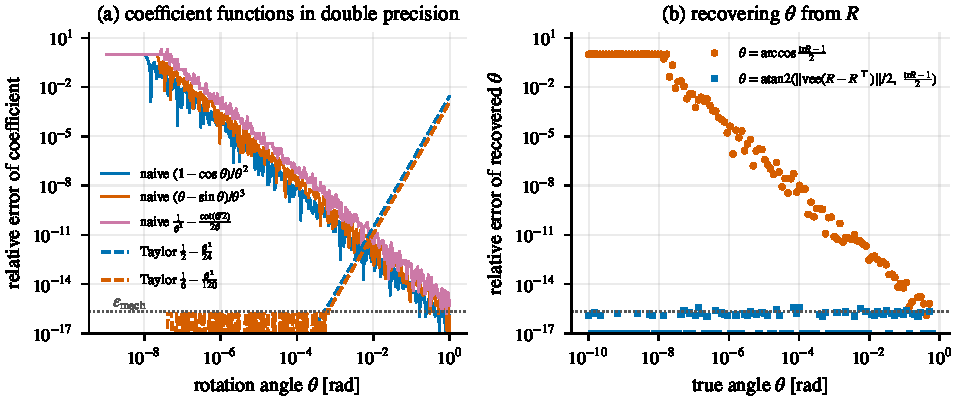
\includegraphics[width=\textwidth]{fig_taylor.pdf}
  \caption{(a) Relative error of the coefficient functions evaluated naively in double precision
  (solid) and with a two-term Taylor series (dashed), against a 60-digit reference. The naive error
  grows like $u/\theta^2$ as $\theta\to0$, and the truncation error of the series grows like $\theta^4$.
  (b) Recovering the angle from a rotation matrix: $\arccos$ loses accuracy like $u/\theta^2$ and
  returns exactly zero below $10^{-8}$, while the $\atantwo$ form is accurate to machine precision at
  every angle.}
  \label{fig:taylor}
\end{figure}

How much does the cancellation matter? It depends on what the coefficient multiplies. A coefficient
with absolute error $\epsilon_c$ that multiplies $\sx{\phi}^k$ contributes an error of about
$\epsilon_c\theta^k$ to the matrix. For $B$, $C$ and $D$, $\epsilon_c \approx u/\theta^2$, so:
\begin{center}\small
\begin{tabular}{@{}l l c l@{}}
\toprule
Function & cancelling coefficient & multiplies & naive absolute error \\
\midrule
$\Exp(\phi)$ & $B$ & $\sx{\phi}^2$ & $\approx u$ \quad (harmless) \\
$\Jr(\phi)$ & $B$ & $\sx{\phi}$ & $\approx u/\theta$ \quad (\textbf{harmful}: $3\times10^{-9}$ at $\theta = 10^{-8}$) \\
$\Jr(\phi)$ & $C$ & $\sx{\phi}^2$ & $\approx u$ \\
$\Jrinv(\phi)$ & $D$ & $\sx{\phi}^2$ & $\approx u$ \\
\bottomrule
\end{tabular}
\end{center}

\begin{keyidea}[why the Taylor branch exists, and how to choose its threshold]
Every function needs a guard against $0/0$. Beyond that, the branch matters for accuracy wherever a
cancelling coefficient multiplies a low power of $\sx{\phi}$, as in $\Jr$. To choose the threshold
$\theta_0$ and the number of terms, balance the two error curves of \cref{fig:taylor}(a): keeping terms
through $\theta^{2m}$ leaves a truncation error of order $\theta^{2m+2}$, and the exact formula has a
rounding error of order $u/\theta^2$. Below the crossing point use the series, above it the formula.
For two-term series ($m = 1$) the curves cross near $\theta \approx 3\times10^{-3}$, where both relative
errors are about $10^{-12}$; adding the $\theta^4$ term moves the crossing to larger angles and lowers
the error there. Remember to multiply by $\theta^k$ when translating a coefficient error into a matrix
error. Record the choice and this justification next to the code (Milestone 2).
\end{keyidea}

% ------------------------------------------------------------------------------
\section{The logarithm map}
\label{sec:log}

\begin{definition}[Logarithm map]
$\Log: \SO \to \R^3$ returns the rotation vector $\phi$ with $\|\phi\| \le \pi$ such that
$\Exp(\phi) = R$.
\end{definition}

For angles strictly between $0$ and $\pi$ the answer is unique. Combining the two equations of
\eqref{eq:trace-angle},
\begin{equation}
  \theta = \atantwo\!\Big( \tfrac12\big\|(R - R\T)\veeop\big\|,\ \tfrac12(\tr R - 1) \Big), \qquad
  \Log(R) = \frac{\theta}{2\sin\theta}\,(R - R\T)\veeop .
  \label{eq:Log}
\end{equation}
The $\atantwo$ form is essential. The common textbook formula $\theta = \arccos\big((\tr R - 1)/2\big)$ is
correct mathematically but numerically unstable near $\theta = 0$, where $\arccos$ has infinite slope,
and loses half the significant digits (\cref{fig:taylor}b). Three regimes need care in code.

\begin{enumerate}
  \item \textbf{Small angles.} $\theta/(2\sin\theta) \to \tfrac12$, so use
        $\Log(R) \approx \tfrac12(1 + \tfrac{\theta^2}{6})(R - R\T)\veeop$.
  \item \textbf{Generic angles.} Use \eqref{eq:Log} directly.
  \item \textbf{Angles near $\pi$.} $\sin\theta \to 0$ and $(R - R\T)\veeop = 2\sin\theta\,u$ vanishes, so
        the axis cannot be recovered from the skew-symmetric part. Use the symmetric part instead: from
        \eqref{eq:rodrigues}, $\tfrac12(R + R\T) = \cos\theta\,I + (1-\cos\theta)\,uu\T$, so
        $uu\T = \big(\tfrac12(R + R\T) - \cos\theta\, I\big)/(1 - \cos\theta)$. Take the column with the largest
        diagonal entry, normalize it to get $\pm u$, and fix the sign so that $u\T(R - R\T)\veeop \ge 0$.
\end{enumerate}

\begin{figure}[t]
\centering
\begin{tikzpicture}[scale=1.0]
  \fill[primarylight] (0,0) circle (2.0);
  \draw[primary, thick] (0,0) circle (2.0);
  \fill (0,0) circle (1.4pt) node[below right] {$I$};
  \draw[->, thick, plotorange] (0,0) -- (1.2,0.8) node[above right=-2pt] {$\phi$};
  \fill[plotgreen] (40:2.0) circle (2pt) node[above right] {$\pi u$};
  \fill[plotgreen] (220:2.0) circle (2pt) node[below left] {$-\pi u$};
  \draw[plotgreen, dashed, <->] (40:1.9) -- (220:1.9);
  \draw[->, plotpurple, thick] (-0.3,-1.2) .. controls (0.6,-1.4) and (1.4,-1.5) .. (330:2.0);
  \draw[->, plotpurple, thick] (150:2.0) .. controls (-1.2,0.6) .. (-0.6,0.4);
  \node[plotpurple, font=\footnotesize, align=left] at (3.6,-1.1) {a path leaving the ball\\re-enters at the\\antipodal point};
  \node[primary, font=\footnotesize] at (0,2.35) {$\|\phi\| \le \pi$};
\end{tikzpicture}
\caption{$\SO$ pictured as the ball of rotation vectors of radius $\pi$, with antipodal points on the
boundary identified ($\pi u$ and $-\pi u$ are the same rotation). $\Log$ is smooth inside the ball but
must jump when a rotation crosses $\theta = \pi$. Near the boundary a tiny change in $R$ can flip the
returned vector to the opposite side.}
\label{fig:so3-ball}
\end{figure}

\begin{remark}[why $\Log$ is ill-conditioned near $\pi$]
Near $\theta = \pi$ two different effects combine. Algebraically, the axis must be extracted from a
nearly vanishing skew-symmetric part, so the na\"ive formula amplifies rounding errors by
$1/\sin\theta$. Topologically, $\Log$ is discontinuous at $\theta = \pi$ (\cref{fig:so3-ball}): a
rotation by $\pi - \epsilon$ about $u$ and one by $\pi - \epsilon$ about $-u$ are close in $\SO$ but have
$\Log$ values $2\pi$ apart. No implementation can remove the second effect. In an estimator it rarely
matters, because $\Log$ is applied to \emph{differences} between nearby rotations, whose angles are
small. Milestone 2 nevertheless tests the near-$\pi$ regime, because a broken branch there produces
\code{NaN}.
\end{remark}

\paragraph{Quaternion logarithm.} For a unit quaternion $q = [w, v]$, first canonicalize to $w \ge 0$ (replace
$q$ by $-q$ if needed), then
\begin{equation}
  \Log_q(q) = 2\,\atantwo(\|v\|, w)\,\frac{v}{\|v\|}
  \ \approx\ \frac{2}{w}\Big(1 - \frac{\|v\|^2}{3w^2}\Big)\,v \quad\text{for small }\|v\|.
  \label{eq:Logq}
\end{equation}
Canonicalization guarantees $\|\Log_q(q)\| \le \pi$ and makes $\Log_q(q) = \Log_q(-q)$, so the double cover is
invisible to the estimator. The $\atantwo$ is well-conditioned at all angles, including near $\pi$ where
$w \approx 0$: the quaternion logarithm does not suffer the algebraic ill-conditioning of the matrix version.
The topological discontinuity at $\pi$ remains.

% ------------------------------------------------------------------------------
\section{The adjoint: moving a perturbation across a rotation}

\begin{proposition}[Adjoint of $\SO$]
\label{prop:adjoint}
For all $R \in \SO$ and $\phi \in \R^3$,
\begin{equation}
  R\,\Exp(\phi)\,R\T = \Exp(R\phi),
  \label{eq:adjoint}
\end{equation}
or equivalently $\Exp(\phi)\,R = R\,\Exp(R\T\phi)$ and $R\,\Exp(\phi) = \Exp(R\phi)\,R$.
\end{proposition}
\begin{proof}
By \eqref{eq:skew-rot}, $R\sx{\phi}R\T = \sx{R\phi}$. By property 4 of \cref{prop:matexp},
$R\exp(\sx{\phi})R\T = \exp(R\sx{\phi}R\T) = \exp(\sx{R\phi})$. The equivalent forms follow by
multiplying on the right or left by $R$ or $R\T$.
\end{proof}

The map $\phi \mapsto R\phi$ is the \emph{adjoint action} $\Ad_R$, which for $\SO$ is simply the rotation
matrix itself. Geometrically, a rotation about an axis $\phi$ expressed in one frame equals the rotation
about the same physical axis expressed in another frame. \Cref{eq:adjoint} is the single most used identity
in Jacobian derivations: it lets you slide a perturbation $\Exp(\delta)$ through other rotations until
it reaches the position the convention requires.

% ------------------------------------------------------------------------------
\section{Composition and the Baker--Campbell--Hausdorff formula}

Rotations about different axes do not commute, so $\Exp(a)\Exp(b) \neq \Exp(a + b)$ in general. The
Baker--Campbell--Hausdorff (BCH) formula quantifies the discrepancy. For matrices $X, Y$ near zero,
\begin{equation}
  \log\big(\exp X \exp Y\big) = X + Y + \tfrac12[X, Y] + \tfrac1{12}\big([X,[X,Y]] + [Y,[Y,X]]\big) + \cdots,
\end{equation}
where $[X, Y] = XY - YX$. For $\so$, \eqref{eq:skew-commutator} gives $[\sx{a}, \sx{b}] = \sx{a\times b}$, so
\begin{equation}
  \Log\big(\Exp(a)\Exp(b)\big) = a + b + \tfrac12\, a\times b
     + \tfrac1{12}\big( a\times(a\times b) + b\times(b\times a)\big) + \cdots .
  \label{eq:bch}
\end{equation}

\begin{proof}[Derivation of the second-order term]
Expand both exponentials to second order: $\exp X\exp Y = (I + X + \tfrac12X^2)(I + Y + \tfrac12Y^2) + O(3) = I + X + Y + \tfrac12X^2 + XY + \tfrac12Y^2 + O(3)$,
where $O(3)$ collects terms of third order in $X$ and $Y$. Write the result as $\exp Z$ with $Z = X + Y + Z_2 + O(3)$ and $Z_2$ of second order. Then
$\exp Z = I + Z + \tfrac12Z^2 + O(3) = I + X + Y + Z_2 + \tfrac12(X + Y)^2 + O(3)$. Comparing the two expansions,
$Z_2 = \tfrac12X^2 + XY + \tfrac12Y^2 - \tfrac12(X^2 + XY + YX + Y^2) = \tfrac12(XY - YX)$. The higher-order terms are obtained the same way, with
more patience; they involve only nested brackets, a theorem in itself.
\end{proof}
The first correction is second order. Two small rotations therefore compose approximately additively,
$\Exp(a)\Exp(b) \approx \Exp(a + b)$, with an error of order $\|a\|\|b\|$. When only one of them is small,
summing the BCH series in the large argument gives the two most important first-order formulas of
this chapter:
\begin{align}
  \Log\big(\Exp(\phi)\,\Exp(\delta)\big) &= \phi + \Jrinv(\phi)\,\delta + O(\|\delta\|^2), \label{eq:bch-right}\\
  \Log\big(\Exp(\delta)\,\Exp(\phi)\big) &= \phi + \Jlinv(\phi)\,\delta + O(\|\delta\|^2), \label{eq:bch-left}
\end{align}
with the Jacobians $\Jr$ and $\Jl$ defined in \cref{sec:jr}.

% ------------------------------------------------------------------------------
\section{Perturbations, \texorpdfstring{$\bplus$}{boxplus} and \texorpdfstring{$\bminus$}{boxminus}}
\label{sec:perturbations}
\label{sec:boxplus}

Let $\hat R$ be an estimate and $R$ the truth. There are two natural ways to write the small rotation
separating them:
\begin{equation}
  \underbrace{R = \hat R\,\Exp(\delta\theta_b)}_{\text{local (right) perturbation}}
  \qquad\qquad
  \underbrace{R = \Exp(\delta\theta_w)\,\hat R}_{\text{global (left) perturbation}} .
\end{equation}
By \cref{prop:adjoint} they describe the same error, related by $\delta\theta_w = \hat R\,\delta\theta_b$.
$\delta\theta_b$ is the error expressed in the estimated body frame, $\delta\theta_w$ the same error expressed in
the world frame. If $\delta\theta_b \sim \N(0, P_b)$, then $\delta\theta_w \sim \N(0, \hat R P_b \hat R\T)$.

\begin{figure}[t]
\centering
\begin{tikzpicture}[scale=1.0]
  % world frame
  \draw[frameaxis, black!60] (0,0) -- (1.1,0) node[right, font=\footnotesize] {$x_w$};
  \draw[frameaxis, black!60] (0,0) -- (0,1.1) node[above, font=\footnotesize] {$z_w$};
  \node[below left, font=\footnotesize] at (0,0) {$W$};
  % estimated and true body frames
  \begin{scope}[shift={(3.4,0.2)}]
    \begin{scope}[rotate=25]
      \draw[frameaxis, primary] (0,0) -- (1.5,0) node[right, font=\footnotesize] {$\hat x_b$};
      \draw[frameaxis, primary] (0,0) -- (0,1.5) node[above left=-2pt, font=\footnotesize] {$\hat z_b$};
    \end{scope}
    \begin{scope}[rotate=45]
      \draw[frameaxis, plotorange, dashed] (0,0) -- (1.5,0) node[above right=-1pt, font=\footnotesize] {$x_b$};
      \draw[frameaxis, plotorange, dashed] (0,0) -- (0,1.5) node[above left=-2pt, font=\footnotesize] {$z_b$};
    \end{scope}
    \draw[->, plotgreen, thick] (25:1.05) arc (25:45:1.05);
    \node[plotgreen, font=\footnotesize] at (35:1.45) {$\delta\theta_b$};
    \node[font=\footnotesize, align=center, below=4pt] at (0.4,0) {estimated frame $\hat R$ (solid)\\ and true frame $R$ (dashed)};
  \end{scope}
  % summary box
  \node[draw=conv, fill=convlight, rounded corners, align=left, font=\footnotesize, text width=5.4cm, anchor=west] at (6.6,0.6) {
    Local: $R = \hat R\Exp(\delta\theta_b)$ \textbf{(this project)}\\[2pt]
    Global: $R = \Exp(\delta\theta_w)\hat R$\\[2pt]
    Same error: $\delta\theta_w = \hat R\,\delta\theta_b$\\[2pt]
    Covariances: $P_w = \hat R P_b \hat R\T$};
\end{tikzpicture}
\caption{The local (right) perturbation measures the attitude error as a small rotation about the axes of
the \emph{estimated} body frame. The global (left) perturbation measures the same error about the world
axes.}
\label{fig:perturbations}
\end{figure}

Both conventions are mathematically valid and widely used, but they are not interchangeable. Every
Jacobian, covariance and residual depends on the choice. The project uses the local one for three
reasons.
\begin{enumerate}
  \item \textbf{It matches the sensor.} The gyroscope measures $\omega_b$ in the body frame and
        \eqref{eq:rdot} puts it on the right, so body-frame errors couple to body-frame quantities.
  \item \textbf{It is decoupled from global yaw.} The local attitude error dynamics
        (\cref{ch:errordyn}) depend on $\hat\omega$ and the biases but not on the absolute heading.
  \item \textbf{It is the convention of the standard ESKF reference~\cite{sola2017quaternion}}, which makes
        the literature easy to cross-check.
\end{enumerate}

\begin{convention}[retraction and local difference, AGENTS.md C4]
For the full state $x = (p, v, q, b_a, b_g, \{p_i, q_i\})$ and $\delta x \in \R^{15 + 6N}$:
\begin{align*}
  x = \hat x \bplus \delta x:&\quad p = \hat p + \delta p,\quad v = \hat v + \delta v,\quad
       q = \hat q\qprod\Exp_q(\delta\theta),\quad b = \hat b + \delta b, \\
  \delta x = x \bminus \hat x:&\quad \delta\theta = \Log_q(\hat q\inv\qprod q),\quad\text{all other blocks subtract.}
\end{align*}
Clone blocks follow the same rule. Every residual, Jacobian, injection and numerical-differentiation test
uses these two operators and nothing else.
\end{convention}

The operators satisfy the axioms that make them a consistent local parameterization:
\begin{equation}
  x \bplus 0 = x, \qquad (x \bplus \delta) \bminus x = \delta, \qquad x \bplus (y \bminus x) = y,
\end{equation}
the second for $\|\delta\theta\| < \pi$ and the third for any $y$. The state is a \emph{product manifold}
$\R^3\times\R^3\times\SO\times\R^3\times\R^3\times(\R^3\times\SO)^N$. Each factor has its own
$\bplus$, and the composite operator acts block-wise.

% ------------------------------------------------------------------------------
\section{Jacobians on manifolds}
\label{sec:jr}

\begin{definition}[Jacobian with respect to local perturbations]
\label{def:manifold-jacobian}
Let $f: \mathcal{M} \to \mathcal{N}$ map between manifolds with $\bplus$/$\bminus$ operators. Its
Jacobian at $x$ is the matrix
\begin{equation}
  J^f_x = \frac{\partial}{\partial\delta}\Big[ f(x\bplus\delta) \bminus f(x) \Big]_{\delta = 0},
  \qquad\text{so that}\qquad f(x\bplus\delta) = f(x)\bplus\big(J^f_x\,\delta + O(\|\delta\|^2)\big).
  \label{eq:manifold-jacobian}
\end{equation}
\end{definition}

When both spaces are vector spaces this is the ordinary Jacobian. The chain rule holds unchanged,
$J^{g\circ f}_x = J^g_{f(x)}\,J^f_x$, so complicated Jacobians are products of simple ones. The column
$j$ of $J^f_x$ is what a finite-difference test computes by perturbing direction $j$, which is how every
such Jacobian is verified.

\subsection{The right and left Jacobians of \texorpdfstring{$\SO$}{SO(3)}}

\begin{definition}[Right and left Jacobians]
The \emph{right Jacobian} $\Jr(\phi)$ is the Jacobian of $\Exp: \R^3 \to \SO$ with the local $\bminus$ on
$\SO$; the \emph{left Jacobian} $\Jl(\phi)$ uses the global one:
\begin{equation}
  \Exp(\phi + \delta) = \Exp(\phi)\,\Exp\big(\Jr(\phi)\,\delta\big) + O(\|\delta\|^2)
  = \Exp\big(\Jl(\phi)\,\delta\big)\,\Exp(\phi) + O(\|\delta\|^2).
  \label{eq:jr-def}
\end{equation}
\end{definition}

$\Jr(\phi)$ answers the question: if I change the rotation \emph{vector} $\phi$ by $\delta$, what small
\emph{body-frame} rotation does the rotation \emph{matrix} undergo? Only for $\phi = 0$ is the answer
$\delta$ itself.

\begin{theorem}[Closed forms]
\label{thm:jr}
With $\theta = \|\phi\|$,
\begin{align}
  \Jr(\phi) &= \int_0^1 \Exp(-s\phi)\,\dd s
             = I - \frac{1-\cos\theta}{\theta^2}\,\sx{\phi} + \frac{\theta - \sin\theta}{\theta^3}\,\sx{\phi}^2, \label{eq:jr}\\
  \Jrinv(\phi) &= I + \tfrac12\sx{\phi} + \Big(\frac{1}{\theta^2} - \frac{1 + \cos\theta}{2\theta\sin\theta}\Big)\sx{\phi}^2, \label{eq:jrinv}\\
  \Jl(\phi) &= \Jr(-\phi) = \Jr(\phi)\T = \Exp(\phi)\,\Jr(\phi), \qquad \Jlinv(\phi) = \Jrinv(-\phi). \label{eq:jl}
\end{align}
The coefficient in \eqref{eq:jrinv} equals $D(\theta) = \frac{1}{\theta^2} - \frac{\cot(\theta/2)}{2\theta}$,
which is finite at $\theta = \pi$ (where $D = 1/\pi^2$) and singular only at $\theta = 2\pi$.
\end{theorem}
\begin{proof}
\emph{Step 1: the derivative of the matrix exponential.} Let $K(t) = \exp\big(t(X + \epsilon Y)\big)$, which solves
$\dot K = (X + \epsilon Y)K$, $K(0) = I$. Its derivative with respect to $\epsilon$ at $\epsilon = 0$, $W(t) = \partial K/\partial\epsilon$, solves the equation obtained by
differentiating the ODE: $\dot W = XW + Y\exp(tX)$, $W(0) = 0$. This is a linear ODE with an input, so by variation of constants
(\cref{prop:stm}) $W(t) = \int_0^t\exp((t - s)X)\,Y\exp(sX)\,\dd s$. At $t = 1$, after substituting $s \to 1 - s$,
\begin{equation*}
  \frac{\dd}{\dd\epsilon}\exp(X + \epsilon Y)\Big|_{\epsilon=0} = \int_0^1 \exp(sX)\,Y\exp((1-s)X)\,\dd s .
\end{equation*}
\emph{Step 2: the integral form.} With $X = \sx{\phi}$ and $Y = \sx{\delta}$,
\begin{align*}
  \Exp(\phi)\inv\,\frac{\dd}{\dd\epsilon}\Exp(\phi + \epsilon\delta)\Big|_0
  &= \int_0^1 \Exp(-(1-s)\phi)\,\sx{\delta}\,\Exp((1-s)\phi)\,\dd s \\
  &= \Big[\int_0^1 \Exp(-s\phi)\,\dd s\ \delta\Big]_\times,
\end{align*}
using $R\sx{\delta}R\T = \sx{R\delta}$ with $R = \Exp(-(1-s)\phi)$ and substituting $s \to 1 - s$ again. Comparing with
$\Exp(\phi)\Exp(\epsilon\Jr\delta) = \Exp(\phi)(I + \epsilon\sx{\Jr\delta}) + O(\epsilon^2)$ gives $\Jr(\phi) = \int_0^1\Exp(-s\phi)\,\dd s$.

\emph{Step 3: the closed form.} With $u = \phi/\theta$, Rodrigues' formula gives
$\Exp(-s\phi) = I - \sin(s\theta)\sx{u} + (1 - \cos(s\theta))\sx{u}^2$. Integrating term by term, $\int_0^1\sin(s\theta)\,\dd s = (1 - \cos\theta)/\theta$ and
$\int_0^1(1 - \cos(s\theta))\,\dd s = 1 - \sin\theta/\theta$, so
$\Jr = I - \frac{1 - \cos\theta}{\theta}\sx{u} + \big(1 - \frac{\sin\theta}{\theta}\big)\sx{u}^2$; substituting $\sx{u} = \sx{\phi}/\theta$ gives \eqref{eq:jr}.

\emph{Step 4: the inverse.} Write $K = \sx{\phi}$, $\Jr = I - BK + CK^2$ with the coefficients $B$ and $C$ of \eqref{eq:jr}, and look for the inverse in the
same form, $I + aK + bK^2$. Multiplying out and reducing $K^3 = -\theta^2K$ and $K^4 = -\theta^2K^2$, the product equals $I$ exactly when
\begin{equation*}
  a - B + \theta^2(bB - aC) = 0, \qquad b - aB + C - \theta^2bC = 0 .
\end{equation*}
These two linear equations have the solution $a = \tfrac12$ and $b = D(\theta)$ (substitute the trigonometric expressions and simplify, or
check numerically), which is \eqref{eq:jrinv}; the identity $\frac{1+\cos\theta}{\sin\theta} = \cot\frac\theta2$ gives the form of $D$.

\emph{Step 5: the left Jacobian.} By \cref{prop:adjoint}, $\Exp(\phi)\Exp(\Jr\delta) = \Exp(\Exp(\phi)\Jr\delta)\Exp(\phi)$, so $\Jl = \Exp(\phi)\Jr$. Repeating
steps 1--3 with the perturbation on the left gives $\Jl = \int_0^1\Exp(s\phi)\,\dd s$, which is $\Jr(-\phi)$ and, since $\Exp(s\phi)\T = \Exp(-s\phi)$,
also $\Jr(\phi)\T$.
\end{proof}

The small-angle expansions are $\Jr(\phi) = I - \tfrac12\sx{\phi} + \tfrac16\sx{\phi}^2 + O(\theta^3)$ and
$\Jrinv(\phi) = I + \tfrac12\sx{\phi} + \tfrac1{12}\sx{\phi}^2 + O(\theta^4)$, with the coefficient series of
\eqref{eq:coeff-taylor}. Equations \eqref{eq:bch-right} and \eqref{eq:bch-left} follow from
\eqref{eq:jr-def} by inverting the relation.

\subsection{Elementary Jacobians}

\begin{table}[t]
\centering\small
\renewcommand{\arraystretch}{1.35}
\begin{tabular}{@{}l l l@{}}
\toprule
Function & Jacobian w.r.t.\ local perturbation & Note \\
\midrule
$f(R) = Rv$ & $\dfrac{\partial f}{\partial\delta\theta} = -R\sx{v}$ & rotate a body vector to world \\
$f(R) = R\T v$ & $\dfrac{\partial f}{\partial\delta\theta} = \sx{R\T v}$ & express a world vector in body \\
$f(R) = R\inv$ & $J = -R$ & output on $\SO$ (local) \\
$f(R_1, R_2) = R_1R_2$ & $J_{R_1} = R_2\T$, \quad $J_{R_2} = I$ & output on $\SO$ (local) \\
$f(\phi) = \Exp(\phi)$ & $J = \Jr(\phi)$ & vector to $\SO$ \\
$f(R) = \Log(R)$ & $J = \Jrinv(\Log R)$ & $\SO$ to vector \\
$f(\phi) = \Exp(\phi)\,v$ & $\dfrac{\partial f}{\partial\phi} = -\Exp(\phi)\sx{v}\Jr(\phi)$ & rotation vector acting on $v$ \\
$f(v) = Rv$ & $J = R$ & ordinary linear map \\
\bottomrule
\end{tabular}
\caption{Elementary Jacobians with respect to the local (right) perturbation $R \to R\Exp(\delta\theta)$. All
other Jacobians in these notes are products of these by the chain rule. Each entry has been checked
numerically by central differences.}
\label{tab:jacobians}
\end{table}

The entries of \cref{tab:jacobians} are derived in two or three lines each. The method is always the same:
\textbf{perturb, expand to first order, isolate the perturbation, and read off the coefficient.}

\begin{example}[Rotation action]
\label{ex:rotation-action}
For $f(R) = Rv$: $f(R\Exp(\delta\theta)) = R(I + \sx{\delta\theta})v + O(\|\delta\theta\|^2) = Rv + R\sx{\delta\theta}v$.
By \eqref{eq:skew-anticomm}, $\sx{\delta\theta}v = -\sx{v}\delta\theta$, so the Jacobian is $-R\sx{v}$.
\end{example}

\begin{example}[Inverse action]
For $f(R) = R\T v$: $(R\Exp(\delta\theta))\T v = \Exp(-\delta\theta)R\T v \approx (I - \sx{\delta\theta})R\T v =
R\T v + \sx{R\T v}\,\delta\theta$.
\end{example}

\begin{example}[Inverse and composition]
For $f(R) = R\inv$: $(R\Exp(\delta\theta))\inv = \Exp(-\delta\theta)R\T = R\T\Exp(-R\delta\theta)$ by
\eqref{eq:adjoint}, so $f(R)\inv f(R\bplus\delta\theta) = \Exp(-R\delta\theta)$ and the Jacobian is $-R$. For
$f = R_1R_2$ perturbed in $R_1$: $R_1\Exp(\delta\theta)R_2 = R_1R_2\Exp(R_2\T\delta\theta)$, so $J_{R_1} = R_2\T$.
Perturbing $R_2$ appends $\Exp(\delta\theta)$ directly, so $J_{R_2} = I$.
\end{example}

\begin{example}[Logarithm]
For $f(R) = \Log(R)$ with $\phi = \Log R$: $\Log(R\Exp(\delta\theta)) = \Log(\Exp(\phi)\Exp(\delta\theta)) \approx
\phi + \Jrinv(\phi)\delta\theta$ by \eqref{eq:bch-right}.
\end{example}

\begin{example}[A chain: a rotation vector acting on a vector]
For $f(\phi) = \Exp(\phi)v$, with $\phi$ an ordinary vector: $\Exp(\phi + \delta)v = \Exp(\phi)\Exp(\Jr\delta)v \approx \Exp(\phi)(v + \sx{\Jr\delta}v)
= \Exp(\phi)v - \Exp(\phi)\sx{v}\Jr(\phi)\delta$. This is the chain rule: the Jacobian of $\Exp$ (namely $\Jr$) followed by the Jacobian of the rotation action
(namely $-R\sx{v}$). It is the Jacobian one needs when a filter uses a rotation vector, rather than a perturbation of a rotation, as its state.
\end{example}

\begin{pitfall}[first-order expansions and products]
The expansion $\Exp(\delta\theta) \approx I + \sx{\delta\theta}$ is valid only when $\delta\theta$ is the
\emph{only} small quantity being differentiated. Products of two small quantities ($\sx{\delta\theta}\delta b$,
or $\sx{\delta\theta}n$ with noise $n$) are second order and are dropped. Large quantities such as the
nominal rotation, the angular rate or the specific force are never approximated.
\end{pitfall}

% ------------------------------------------------------------------------------
\section{Uncertainty on \texorpdfstring{$\SO$}{SO(3)}}

With the local perturbation, an uncertain attitude is the random rotation
\begin{equation}
  R = \hat R\,\Exp(\delta\theta), \qquad \delta\theta \sim \N(0, P_\theta),
\end{equation}
a ``Gaussian on the manifold'': the mean $\hat R$ lives on $\SO$ and the covariance $P_\theta$ lives in the
tangent space at $\hat R$, in body-frame coordinates. Its eigenvectors are body axes about which the
attitude is most or least certain. This distribution is not a Gaussian in any fixed coordinates of
$\SO$, which is exactly why it captures curved distributions such as the banana of \cref{fig:banana}
better than a Gaussian on Euler angles or matrix entries.

\paragraph{Propagation.} If $y = f(R)$ and $J$ is its manifold Jacobian, then to first order
$y = f(\hat R)\bplus\delta y$ with $\delta y \approx J\delta\theta \sim \N(0, JP_\theta J\T)$.

\paragraph{Compounding.} For independent uncertain rotations $R_1 = \hat R_1\Exp(\delta_1)$ and
$R_2 = \hat R_2\Exp(\delta_2)$, the composition is
$R_1R_2 = \hat R_1\hat R_2\Exp(\hat R_2\T\delta_1)\Exp(\delta_2) \approx \hat R_1\hat R_2\Exp(\hat R_2\T\delta_1 + \delta_2)$, so
\begin{equation}
  P_{12} = \hat R_2\T P_1\hat R_2 + P_2 .
\end{equation}

\begin{remark}[covariance entries rotate between axes]
\label{rem:cov-rotates}
Because $P_\theta$ is expressed in body axes, it changes when the body rotates even if no information is
gained or lost. Suppose the world yaw is uncertain and roll and pitch are perfectly known: in world
coordinates $P_w = \sigma^2 e_ze_z\T$. In body coordinates $P_b = \hat R\T P_w\hat R = \sigma^2 (\hat R\T e_z)(\hat R\T e_z)\T$.
If the vehicle rolls by $90^\circ$, the world vertical is the body $y$-axis, and the yaw uncertainty moves
from the $(z,z)$ to the $(y,y)$ entry of $P$. Individual diagonal entries of the attitude covariance
are therefore not monotonic during propagation (a Milestone 5 concept), although its trace and
eigenvalues behave as expected.
\end{remark}

\subsection{Averaging rotations}

\index{rotation averaging}
How should several noisy measurements $R_1, \dots, R_N$ of the same attitude be averaged? The arithmetic mean of matrices (or of
quaternions) is not a rotation, and the average of Euler angles is meaningless near wrap-around. The natural definition is the rotation that
minimizes the sum of squared tangent-space distances, $\bar R = \argmin\sum_i\|\Log(\bar R\T R_i)\|^2$. It is computed by the fixed-point iteration
\begin{equation}
  \bar R \gets \bar R\,\Exp\Big(\frac1N\sum_{i=1}^N\Log\big(\bar R\T R_i\big)\Big),
\end{equation}
which averages the residuals in the tangent space at the current estimate and moves the estimate by that average, exactly as one would
average vectors, but on the manifold. It converges in a few iterations when the rotations are within a few tens of degrees of each other.
A faster approximation projects the arithmetic mean $M = \frac1N\sum_iR_i$ onto $\SO$ with the SVD: if $M = U\Sigma V\T$, the closest rotation is
$U\diag(1, 1, \det(UV\T))V\T$ (the same construction as in \cref{sec:umeyama}).

% ------------------------------------------------------------------------------
\section{\texorpdfstring{$\SE$}{SE(3)} and the choice of state manifold}
\label{sec:se3}

The rigid transformations $T = \begin{bmatrix}R & p\\0 & 1\end{bmatrix}$ of \cref{ch:rotations} also form a Lie group, $\SE$, of dimension six.

\paragraph{Lie algebra.} Differentiating a curve $T(t)$ through the identity gives elements of the form
$\xi\hatop = \begin{bmatrix}\sx{\phi} & \rho\\ 0 & 0\end{bmatrix}$, parameterized by $\xi = (\rho, \phi) \in \R^6$: an angular velocity $\phi$ and a linear velocity $\rho$,
together a \emph{twist}.

\paragraph{Exponential.} The powers of $\xi\hatop$ are $\begin{bmatrix}K^k & K^{k-1}\rho\\0 & 0\end{bmatrix}$ for $k \ge 1$, with $K = \sx{\phi}$, so the exponential series gives
\begin{equation}
  \Exp(\rho, \phi) = \begin{bmatrix}\Exp(\phi) & \Jl(\phi)\,\rho \\ 0 & 1\end{bmatrix},
  \qquad \Jl(\phi) = \sum_{k\ge0}\frac{K^k}{(k + 1)!},
\end{equation}
where the series is the left Jacobian of \cref{thm:jr} (expand $\int_0^1\Exp(s\phi)\,\dd s$ term by term). Moving with a constant twist traces a
\emph{screw motion}: rotation about an axis combined with translation along it. The logarithm inverts the two blocks: $\phi = \Log(R)$ and
$\rho = \Jl(\phi)\inv p$.

\paragraph{Adjoint.} Conjugation $T\Exp(\xi)T\inv = \Exp(\Ad_T\xi)$ holds with the $6\times6$ matrix
\begin{equation}
  \Ad_T = \begin{bmatrix} R & \sx{p}R \\ 0 & R \end{bmatrix},
\end{equation}
obtained by multiplying out $T\xi\hatop T\inv$. It transforms twists between frames, and plays the same role for poses as $R$ does for rotation vectors.

\paragraph{Which manifold for the state?} Perturbing a pose on $\SE$, $T = \hat T\Exp(\delta\xi)$, expresses the translation error in the body frame
and couples it to the rotation error through $\Jl$. The project does \emph{not} do this: its state is the product manifold of
\cref{sec:boxplus}, in which the position error is a plain world-frame vector and the attitude error is a local rotation, independently.
To first order the two are related by a rotation of the translation error ($\delta p_w \approx \hat R\,\delta\rho$); they differ at second order. Both
choices are valid, but they produce different Jacobians and different covariances, and must never be mixed. A third choice, the
extended pose group $\mathrm{SE}_2(3)$ of $5\times5$ matrices $\begin{bmatrix}R & v & p\\0 & 1 & 0\\0 & 0 & 1\end{bmatrix}$ collecting attitude, velocity and
position, underlies the \emph{invariant} EKF, whose error dynamics have the striking property of not depending on the state at all
(\cref{ch:observability}).

% ------------------------------------------------------------------------------
\section{Verifying manifold Jacobians numerically}
\label{sec:numjac}

Every analytic Jacobian in the project is checked against a central difference built on the
$\bplus$/$\bminus$ operators (AGENTS.md E6). Column $j$ of the numerical Jacobian is
\begin{equation}
  J_{:,j} \approx \frac{ f(x\bplus h e_j) \bminus f(x\bplus(-h e_j)) }{2h},
  \qquad h \approx 10^{-6}.
  \label{eq:numjac}
\end{equation}
The central difference has truncation error $O(h^2)$ and rounding error $O(u/h)$
(\cref{sec:numdiff}), so analytic and numerical Jacobians should agree to about $10^{-8}$ relative
to the magnitude of the entries.

\begin{pitfall}[tests that cannot fail]
A Jacobian test evaluated at a trivial point proves little. At $R = I$, $R$ and $R\T$ are equal, so a
transpose bug is invisible; with zero angular rate, terms multiplied by $\hat\omega$ vanish; with zero
biases, bias-sign errors may hide. Always test at a random non-identity attitude, non-zero rates,
accelerations and biases, and ask of every test: \emph{would this still pass if I flipped the sign of
X?} A good habit is to temporarily break the analytic Jacobian and confirm that the test fails.
\end{pitfall}

\begin{projectlink}[Milestone 2]
\code{so3.hpp} implements \code{skew}, \code{Exp}/\code{Log}, \code{Exp\_q}/\code{Log\_q}, \code{J\_r} and
\code{J\_r\_inv} as derived here, and \code{numerical\_jacobian.hpp} implements \eqref{eq:numjac} generically
over $\bplus$/$\bminus$. The exit criteria test exactly the properties of this chapter: $\Exp(\phi) \in \SO$,
$\Log\circ\Exp = \mathrm{id}$ at zero, tiny, generic and near-$\pi$ angles, agreement of $\Exp_q$ and $\Exp$,
$\Log_q(q) = \Log_q(-q)$, the defining relation \eqref{eq:jr-def} of $\Jr$, and $\Jrinv\Jr = I$, all
without allocation.
\end{projectlink}

\begin{takeaways}
\begin{itemize}
  \item Attitude lives on the curved manifold $\SO$; its errors live in the flat tangent space $\R^3$.
        $\Exp$ and $\Log$ connect them.
  \item Compute angles with $\atantwo$, never with $\arccos$. Guard every coefficient function against
        $0/0$, and use Taylor branches wherever cancellation is amplified (notably in $\Jr$).
  \item Local (right) perturbation: $R = \hat R\Exp(\delta\theta)$, error in body axes. Global errors are
        $\hat R\,\delta\theta$.
  \item The adjoint identity $R\Exp(\phi)R\T = \Exp(R\phi)$ moves perturbations through rotations.
  \item $\Exp(\phi + \delta) \approx \Exp(\phi)\Exp(\Jr(\phi)\delta)$ and
        $\Log(\Exp(\phi)\Exp(\delta)) \approx \phi + \Jrinv(\phi)\delta$.
  \item Every project Jacobian is a chain-rule product of the entries of \cref{tab:jacobians}, and is
        verified by central differences at a non-trivial point.
\end{itemize}
\end{takeaways}

\begin{exercises}
  \item Show that $\so$ is closed under the commutator $[X, Y] = XY - YX$ and that
        $[\sx{a}, \sx{b}] = \sx{a\times b}$.
  \item Prove $\Exp(-\phi) = \Exp(\phi)\T$ and $\Exp(s\phi)\Exp(t\phi) = \Exp((s+t)\phi)$. Why does the second
        identity not contradict non-commutativity?
  \item Implement $\Log$ with both $\arccos$ and $\atantwo$ and reproduce \cref{fig:taylor}(b).
        Then construct a rotation within $10^{-6}$~rad of $\pi$ and test the near-$\pi$ branch.
  \item Using the coefficient series of \eqref{eq:coeff-taylor}, choose a threshold and a number of terms
        for $\Jr$ so that its absolute error stays below $10^{-14}$ for all $\theta \in [0, 0.1]$. Justify
        your choice with the error model of \cref{sec:taylor}.
  \item Derive the Jacobian of $f(R) = \Log(\hat R\T R)$ with respect to a local perturbation of $R$, and of
        $g(\hat R) = \Log(\hat R\T R)$ with respect to a local perturbation of $\hat R$. Evaluate both at
        $R = \hat R$. (These are the building blocks of attitude residuals.)
  \item Show that $\Jl(\phi) = \Exp(\phi)\Jr(\phi)$ and use it to prove \eqref{eq:bch-left} from
        \eqref{eq:bch-right}.
  \item A vehicle has attitude covariance $P_b = \diag(\sigma_r^2, \sigma_r^2, \sigma_y^2)$ in body axes while
        level. Compute $P_b$ after it pitches by $90^\circ$ with no new information, and interpret.
  \item Verify every row of \cref{tab:jacobians} with a 20-line Python script using central differences at
        a random point. Then flip one sign and confirm your script detects it.
\end{exercises}
